\newglossaryentry{Charles D. Moore}
{
  name={Charles D. Moore},
  description={Charles D. Moore, is the inventor of the forth programming language.}
}

\chapter{Results}
\label{chap:Results}

In this chapter, I will introduce the chosen forth software. Afterwards, I will manually or semi automatically produce the graphics according to the selected Visualization methods.

\section{The software under investigation: Brainless}

Brainless\footnote{Brainless verion 0.1.2 is used, the source code can be optained on \url{http://sourceforge.net/projects/forth-brainless/}} is chess-playing program written in ANS Forth. The source code consists of several files with an overall size\footnote{The command to calculate the size was \emph{find . -name '*.fs' -maxdepth 1 | xargs wc -l}} of 139497 bytes and 4108 lines of code\footnote{The command used to count the lines of code, was \emph{find . -name '*.fs' -maxdepth 1 | xargs wc -l}}.
This measure is somehow controversial, but since the files contain only a short header and are formatted in the usual manner, it seems appropriate for comparison. The code is organized in a flat structure. There is one directory with 30 files, which contain 663 words. There is only one custom word list defined. Thus the visualization of a word list hierarchy makes obviously little sense and is left out in the following sections.

The other software, I took into consideration, was brew\footnote{brew version 0.2.0 was used. The source code can be obtained on \url{http://www.robertepprecht.ch/brew/index.html}}. Brew is a 'playground for evolutionary programming', as the author calls it. Due to its size of 1062857 bytes and 36801 lines of code, this project seem to large to analyze manually in a reasonable time.

For the following figures, I used a snapshot of an execution trace.
Since the calculations of the computer-moves produce a huge amount of word executions, the example trace, was created by making only the player-move: \emph{d2 d3 m} \keys{\return}. The snapshot contains all word executions after and including the execution of the word \emph{m}. It consists of 4709 word executions. \ref{fig:brainless_before_m} and \ref{fig:brainless_after_m} show the state of the game before and after entering \emph{d2 d3 m} \keys{\return}.

\begin{figure}[p]
    \centering
    \includegraphics[scale=0.4]{graphics/brainless_before.png}
    \caption{State of the game before entering \emph{d2 d3 m}}
    \label{fig:brainless_before_m}
\end{figure}

\begin{figure}[p]
    \centering
    \includegraphics[scale=0.4]{graphics/brainless_after.png}
    \caption{State of the game after entering \emph{d2 d3 m}}
    \label{fig:brainless_after_m}
\end{figure}

\section{The application of the previously presented methods}

\subsection*{Hierarchical edge bundles}

Figure \ref{fig:hierarchic_edge_bundle} shows the first 100\footnote{The calculation of the interaction lines consume a considerable amount of system resources, which prevents longer traces due to memory limitation.} word executions of the trace snapshot mentioned before in a \emph{hierarchic edge bundle}.

The outer ring labeled with \emph{brainless-0.1.2} represents the directory of the source code, the middle ring represents the files and the inner ring represents the words. Words which haven't been executed in this snapshot, have been omitted.
The word sectors are of equal angle, the number of different words divided by 360\degree. The file sectors' angle have been adjusted according to the number of files they contains.
The lines in the circle represent word executions. Same as in \cite{Holten:2006:HEB:1187627.1187772}, the word on the green end is the caller and the word on the red end is the callee. The distance of the turning point to the center of the circle depends on the distance(in degree) of the two word sectors, words with great distance are connected near to center. Multiple occurrences of caller/callee pair appear as one line in this graph. The exact algorithms used to calculate \ref{fig:hierarchic_edge_bundle} can be found in \hl{<appendix>}.
A further improvement would be to draw multiple occurrences of the same caller/callee pairs with a slight gap to visualize all the executions.

<The interpretation>

\begin{figure}[p]
    \centering
    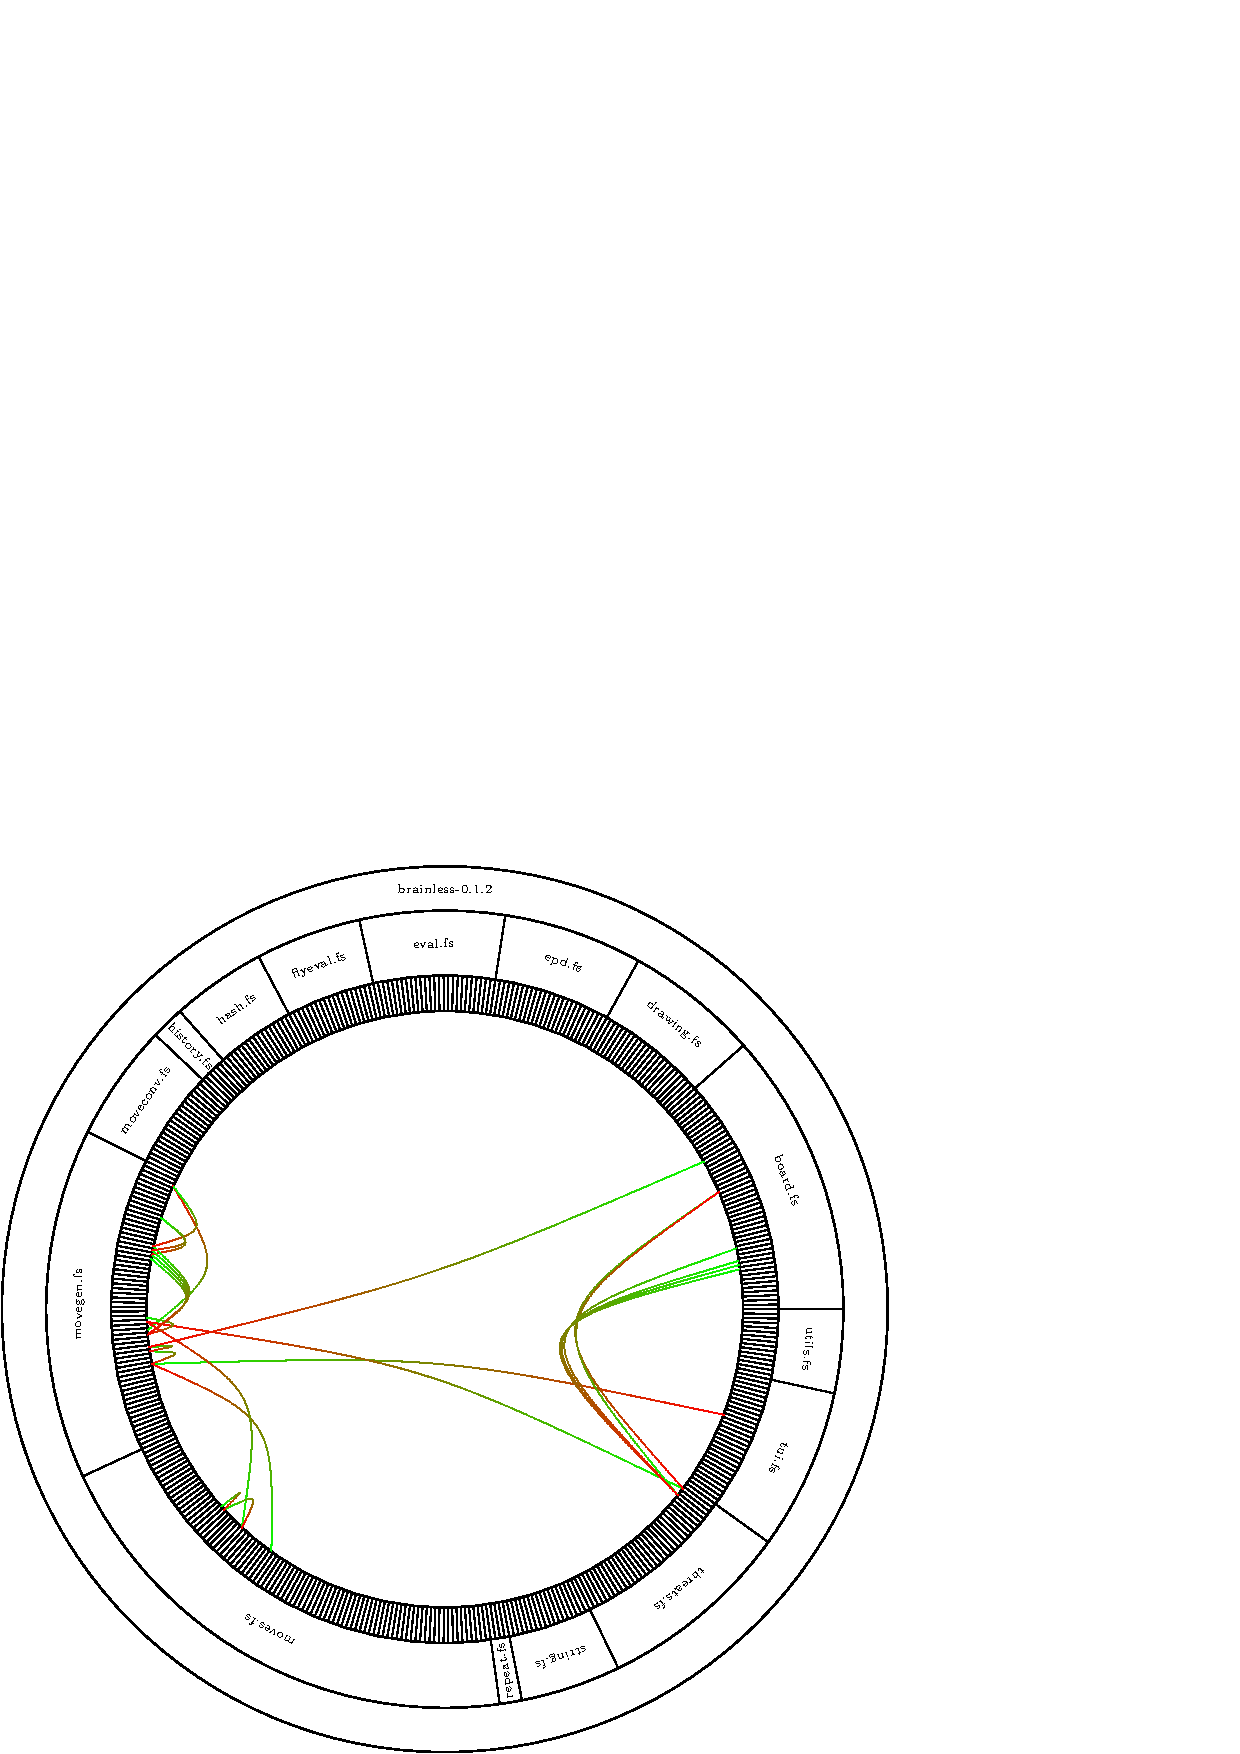
\includegraphics[scale=0.65]{graphics/hierarchic_edge_bundle-dir_file_word.png}
    \caption{Hierarchic edge bundle of a small snapshot of the trace of Brainless after \emph{d2 d3 m}}
    \label{fig:hierarchic_edge_bundle}
\end{figure}


\subsection*{Information murals and massive sequence view}

Figures \ref{fig:massive_sequence_view_1}, \ref{fig:massive_sequence_view_2} and \ref{fig:massive_sequence_view_3} show the trace snapshot in a \emph{massive sequence view}.

The \emph{massive sequence view} consists of a hierarchical part at the top of \ref{fig:massive_sequence_view_1} and the interaction part which follows immediately(\ref{fig:massive_sequence_view_2} and \ref{fig:massive_sequence_view_3}). The upper level of the hierarchical part labeled with \emph{brainless-0.1.2}, again, represents the directory of the source code. The middle level, the files and the lower level, the words. Again, words which haven't been executed in this snapshot, have been omitted.
The interaction part shows the word executions as lines. As in \cite{Holten:2006:HEB:1187627.1187772}, the word above the green end is the caller and the word above the red end is the callee. The order of the interaction lines represents also the order of execution. The first executed word is represented by the upper most interaction line.

<The interpretation>
It is easy to identify certain steps of the program execution like the drawing part at the end of the trace(interaction with drawing.fs shown if figure \ref{fig:massive_sequence_view_2}) and the file writing part(interaction from epd.fs at the and of figure \ref{fig:massive_sequence_view_2}), if one know the words contained in those files. But it also clearly shows the lack of interactivity. Without filtering, zooming, on-demand information on words(references to source code) and of course expressive naming, it still remains hard to map the sections of the trace to behavior. Besides these concerns, the massive sequence view seems to be well applicable to forth program traces.

\begin{figure}[p]
    \centering
    \includegraphics[scale=0.52]{graphics/massive_sequence_view-dir_file_word_1.png}
    \caption{Massive sequence view(Part 1) of Brainless after \emph{d2 d3 m}}
    \label{fig:massive_sequence_view_1}
\end{figure}

\begin{figure}[p]
    \centering
    \includegraphics[scale=0.52]{graphics/massive_sequence_view-dir_file_word_2.png}
    \caption{Massive sequence view(Part 2) of Brainless after \emph{d2 d3 m}}
    \label{fig:massive_sequence_view_2}
\end{figure}

\begin{figure}[p]
    \centering
    \includegraphics[scale=0.52]{graphics/massive_sequence_view-dir_file_word_3.png}
    \caption{Massive sequence view(Part 3) of Brainless after \emph{d2 d3 m}}
    \label{fig:massive_sequence_view_3}
\end{figure}

\subsection*{High-Level polymetric views}

Figure \ref{fig:polymetric_view} shows a polymetric view of the snapshot. 
I used a circle to represent a single word. The radius reflects the number of executions, frequently executed words appear as larger circles. The position(distance from the origin) reflects the number of words executed within the word, fewer sub-word-executions result in a greater distance. If the number of sub executions vary, the maximum was used. The color of a circle reflects the io-behavior of a word. Red means, the word prints to stdout and yellow means it is reading from or writing to a file.

<The interpretation>
\hl{TODO gro�e w�rter = performance relevant, w�rter die in der mitte sind, sind eher intern komplex, farben: w�rter die tats�chlich was sichtbares tun}

\begin{figure}[p]
    \centering
    \includegraphics[scale=0.55]{graphics/polymetric_view.png}
    \caption{High-Level polymetric view of the trace of Brainless after \emph{d2 d3 m}}
    \label{fig:polymetric_view}
\end{figure}

\subsection*{Memory access view}

Figure \ref{fig:taxonomy} shows a small snapshot of the memory access of brainless.
It shows the words and the memory locations they access. The words are represented by circles and the memory locations(values) by rectangles. The arrows represent the direction of the access. An outgoing arrow(from a word to a memory location) represents write operation and an incoming arrow(from a memory location to a word), a read operation.
Since Brainless makes extensive use of \emph{value}s, does not use *\emph{variable}s at all and uses custom defining words only occasionally, \ref{fig:taxonomy} shows only the \emph{value}s.

<The interpretation>
It should cover \emph{value}, \emph{variable}, \emph{2variable}, \emph{fvariable} and also memory fields, allocated by custom defining words.

\begin{figure}[p]
    \centering
    \includegraphics[scale=0.20]{graphics/taxonomy_view2.png}
    \caption{Snapshot of the memory access of Brainless}
    \label{fig:taxonomy}
\end{figure}

\section{gfvis - A trace visualization enhancement for Gforth}

\hl{TODO put this under the matching viz methods!!}
A very important question in this concern is, how can developers be assisted to write readable code. Experienced developers may do that intuitively, but how can novice developers be encouraged and supported to write readable code. Concatenative languages are flexible enough to produce code very similar to natural languages, but how can this attribute be supported?\\
One answer is to provide hints based on static analysis.\\
It is not possible to make every word completely readable and the perceived readability also depends on the experience of the developer. At some point  it always comes down to longer combinations of "nip tuck over rot", this is hardly avoidable at the lowest level. Thus, proper documentation of words is essential. It is pretty obvious, that stack effect comment\footnote{See \url{https://www.complang.tuwien.ac.at/forth/gforth/Docs-html/Stack\_002dEffect-Comments-Tutorial.html\#Stack\_002dEffect-Comments-Tutorial}} in Forth, are a must have, but also the behavior of the word should be documented for complex or not very natural to read words\footnote{Most notable \\G in Gforth. See \url{https://www.complang.tuwien.ac.at/forth/gforth/Docs-html/Comments.html\#Comments}}. Another advantage of word definition comments is the possibility of automated documentation generation.\\
Very long word definitions tend to increase the amount of brain capacity required to understand its behavior. A way to address this problem is to break down the overall task into small, manageable pieces. In context of concatenative languages, this is called factoring\footnote{See \url{https://www.complang.tuwien.ac.at/forth/gforth/Docs-html/Factoring-Tutorial.html\#Factoring-Tutorial}} in context of concatenative languages. One approach could be to place a hint on word definitions which exceed a certain amount of lines or words or different words and suggest further factoring.\\
Another tool to make code reading more natural, is aliasing\footnote{See \url{https://www.complang.tuwien.ac.at/forth/gforth/Docs-html/Aliases.html}}. By defining aliases for a certain word, its functionality can be used in different contexts and still read very natural.
Although obvious, it should be mentioned that assigning expressive and fitting names for words is essential.\\
To understand code, the systematic approach turned out to be most efficient\cite{Robillard:2004:EDI:1042203.1042417}. To ease afford of finding the definition of words used at a certain point, a hyperlink like referencing mechanism can be used[cite the visualization paper with the hyperlink feature].\\
As stated by \gls{Charles D. Moore} in \cite{Biancuzzi:2009:MPC:1592983}: "... The challenge there is 1) deciding
which words are useful, and 2) remembering them all.", when programs get larger, the amount of words can grow big. Thus it is suggested to have some sort of a dictionary to search the whole vocabulary by name, stack effect comment, word definition documentation and provide a reverence to where they are used. Auto completion can also help a lot in finding words previously defined.

\begin{itemize}

\item other data structures and variables should be displayed
	\begin{itemize}
	\item memory maybe like \cite{ReissProgrammingEnvironments1995} or \cite{Aftandilian:2010:HIH:1879211.1879222} but since there is no underlying object orientation and no standardized oo system this would be hard do accomplish
	\item fisheye or word cloud like display(tree or sugiyama as of \cite{Storey:1997:IVT:857188.857642})
	\end{itemize}


\item interactive program manipulation: state of the system before a word, after a word and by clicking on the word jumping to its definition or inserting it and there also providing those features

\item stepping debugger mode: simply stepping through the whole code word by word

\item goal-oriented strategy: the definition of an execution scenario such that only the parts of interest of the software system are analyzed (Koenemann and Robertson, 1991; Zaidman,
2006).

\item code analysis and visualization facilities see chapter 2 TODO
\end{itemize}

\subsection{software maintenance}

\begin{itemize}
\item types of maintenance
\item find bugs and fix them
\item find the right place to implement a new feature.
\item find the right place to modify a feature.
\end{itemize}

\subsection{program comprehension}

\begin{itemize}
\item structured approach
\item thorough reading is the most efficient[cite]
\item about the mental model building
\item keeping the mental model up to date
\item keeping artifacts up to date
\end{itemize}


